\subsection{Taylor Series - Chapter 4}

\begin{enumerate}

\item {\bf First Order Approximation - Euler's Method}

Euler's Method of Integration is a method used to integrate
equations of motion. Because the method is first order, Euler's
method tends to be largely inaccurate. The basic idea of Euler's
Method is to approximately determine a function $f$ while only
knowing $\dot{f}=\frac{df}{dt}$. That is, it is beneficial to integrate
$\dot{f}$ to obtain $f$. If we plot a general plot of f(t) we
obtain the graph above.
\begin{figure}[H]
  \begin{center}
    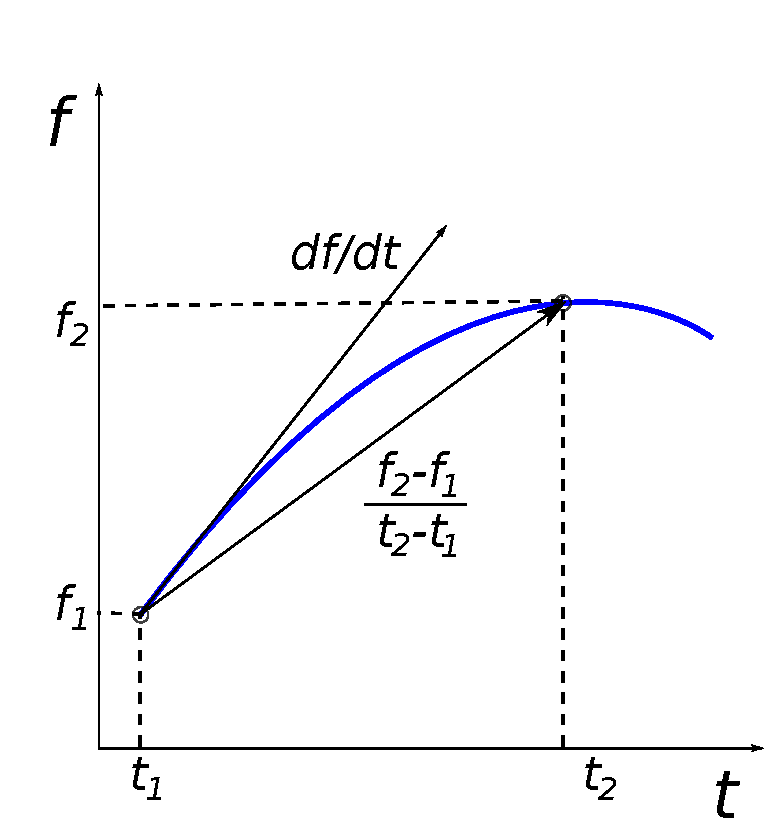
\includegraphics[height=0.5\textwidth,width=0.5\textwidth]{Graphics/Eulers_Method.pdf}
  \end{center}
\end{figure}
Here, the blue line is the analytical equation for $f$. Using this
graph it is possible to write that

\begin{equation}
  \dot{f}_1 \approx \frac{f_2-f_1}{t_2-t_1}
\end{equation}

if we then use the relationship that $t_2 = \Delta t + t_1$ we can
write that 

\begin{equation}
  \dot{f}_1 \approx \frac{f_2-f_1}{\Delta t}
\end{equation}

Note that in the limit as $\Delta t \rightarrow 0$ we have

\begin{equation}
  \lim_{\Delta t \rightarrow 0} \frac{f_2-f_1}{\Delta t} = \dot{f}_1
\end{equation}

thus as we reduce our timestep in our measurement we create a more
and more accurate representation of $f$. Returning to our
approximate equation for $\dot{f}$ we can rearrange this equation
to write.

\begin{equation}
  f_2 \approx f_1 + \dot{f}_1\Delta t 
\end{equation}

Thus the value of $f_2$ can be estimated if the derivative and the
initial value are known. It is simple to extrapolate to another
timestep such that

\begin{equation}
  f_3 \approx f_2 + \dot{f}_2\Delta t
\end{equation}

Thus as long as the derivative of $f$ and the initial condition is
known, $f$ can be numerically integrated using the recursive
algorithm.

\begin{equation}
  f_{i+1} \approx f_i + \dot{f}_i\Delta t
\end{equation}

\item{\bf The Series}

Recall that Euler's method uses a simple approximation for the
derivative using simple forward differencing. That is,

\begin{equation}
\frac{df}{dt} \approx \frac{f_{i+1} - f_i}{t_{i+1} - t_i}
\end{equation}

We then said that $f(t_{i+1}) = f(t_i) + \dot{f}(t_i)\Delta t$. This
is a first order approximation to the function f. It is possible to
create higher order approximations using more terms such that

\begin{equation}
f(t_{i+1}) \approx f(t_i) + f'(t_i)\Delta t +
f''(t_i)\frac{\Delta t^2}{2!} +
f'''(t_i)\frac{\Delta t^3}{3!} + ... + f^{(N)}(t_i)\frac{\Delta t^N}{N!}
\end{equation}

\item{\bf Error}

The Taylor series always contains error since it is impossible to
compute an infinite series. The easiest way to derive the error is by
way of logical extension. If we write the zero order approximation to
$f$ we have

\begin{equation}
f(t_{i+1}) \approx f(t_i)
\end{equation}

our error would then be 

\begin{equation}
R_0 \approx f'(t_i)\Delta t + f''(t_i)\frac{\Delta t^2}{2!} +
f'''(t_i)\frac{\Delta t^3}{3!} + ... + f^{(N)}(t_i)\frac{\Delta t^N}{N!}
\end{equation}

however graphically we can show that in fact our error can simply be
written as

\begin{equation}
R_0 = f'(\zeta)\Delta t
\end{equation}

using the graph below.

\begin{figure}[H]
  \begin{center}
    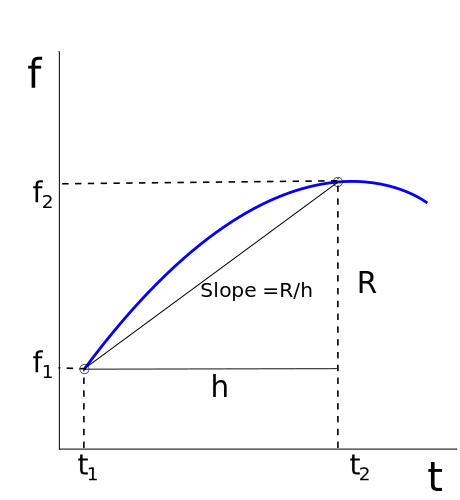
\includegraphics[height=0.45\textwidth,width=0.45\textwidth]{Graphics/Taylor_Series_Error}
  \end{center}
\end{figure}

where $\zeta$ is a number between B and A. It is easy to extend this
to $R_1 = f''(\zeta)\Delta t^2/2!$ or generally

\begin{equation}
R_N = \frac{f^{(N+1)}(\zeta)\Delta t^{N+1}}{(N+1)!}
\end{equation}

\item{\bf The Non-linear Parachutist}

  Let's return to the parachutist. In that problem we had

  \beq
  \dot{v}+(c/m)v=g
  \eeq

  Since the drag was Newtonian the analytical solution could be
  obtained using simple differential equation techniques.

  \beq
  v(t) = v_0e^{-ct/m}+(1-e^{-ct/m})mg/c
  \eeq

  However, if Bernoulli drag is used instead the equations of motion
  become

  \beq
  \dot{v}+(c/m)v^2=g
  \eeq

  This unfortunately has no analytical solution. The solution then is
  to solve the problem numerically using Euler's method. If the
  initial condition is known $v_0$ the problem reduces to the
  following equations

  \beq
  \begin{matrix}
  \dot{v}_0 = g-(c/m)v^2_0\\
  v_1 = v_0 + \dot{v}_0\Delta t\\
  \dot{v}_1 = g-(c/m)v^2_1\\
  v_2 = v_1 + \dot{v}_1\Delta t\\
  \vdots\\
  \dot{v}_N = g-(c/m)v^2_N\\
  v_{N+1} = v_N + \dot{v}_N\Delta t\\
  \end{matrix}
  \eeq

  Provided the timestep is small enough the solution will converge to
  the actual solution.

 
\end{enumerate}
